\vspace{-4mm}
\begin{figure}[htbp]
  \centering
  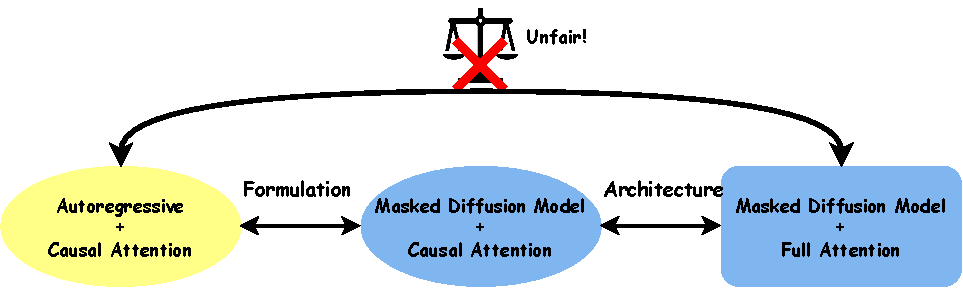
\includegraphics[width=0.8\linewidth]{plots/fair_comparison.drawio.pdf}
  \label{fig:example}
\end{figure}
\vspace{-2mm}
\section{Introduction}
The pursuit of more powerful and efficient foundation models drives continuous exploration beyond dominant autoregressive (AR) methods for language modeling.
The remarkable success of diffusion models~\cite{sohl2015deep,ho2020denoising,song2020score} in continuous domains has naturally spurred investigation into the viability and potential benefits of discrete diffusion models~\cite{austin2021structured,campbell2022continuous,lou2023discrete} for language modeling. 
Among the strategies emerging within the discrete diffusion framework, masked (absorbing state) diffusion models (MDMs) have captured considerable attention. Recent works such as LLaDA~\cite{nie2025large} and Dream~\cite{dream2025} have successfully scaled these masked diffusion models to 7B parameters, achieving compelling results that challenge the sole dominance of AR methods.

Yet, in comparisons between AR and MDM paradigms, a fundamental \textit{architectural difference} is often overlooked: the former typically operates within a \textit{causal attention, decoder-only} setting, whereas the latter commonly employs \textit{full attention} within an \textit{encoder-only} setup.
Beyond the high-level paradigm, the choice between causal and full attention dictates significant differences in training, density estimation, and generation efficiencies. Intriguingly, recent studies such as ENTP~\cite{ewer2024entp} and MAR~\cite{li2024autoregressive} provide evidence hinting that full attention, despite its typical association with non-causal tasks, might hold inherent theoretical advantages and achieve superior empirical results even in contexts aiming for sequential, AR-like generation. This highlights the need to decouple the effects of the theoretical formulations (AR vs. MDM) from the underlying attention mechanism.

Building upon this observation, we propose and evaluate MDMs (as Any-Order AR) implemented within a decoder-only framework, a deliberate choice to enable a more equitable comparison against conventional autoregressive models. This setup allows us to isolate variables and answer the following two questions: 
\begin{enumerate}
    \item Within decoder-only architecture, what are the differences in modeling capabilities and empirical performance when using AR versus MDM formulation for language tasks?
    
    \item Within the MDM framework for language tasks, what are the theoretical and empirical differences when selecting an encoder-only versus a decoder-only architecture?
\end{enumerate}
To answer these questions, we specifically design AO-GPT\footnote{In this paper, AO-AR refers to the generative formulation, which can be implemented with either encoder-only or decoder-only architectures. In contrast, AO-GPT specifically denotes our model that combines the AO-AR objective with a decoder-only architecture.}, a decoder-only architecture capable of modeling any-order sequences, with the potential to unify AR and MDM in a single model. We then conduct a series of carefully designed experiments. In Section~\ref{sec:decoder ar vs mdm}, we delve into the first question by systematically investigating the impact of varying the distribution over token prediction orders during training, while keeping the decoder-only architecture constant. Our analysis in this section, leading to Findings 1-3, aims to clarify some intrinsic characteristics of language data, convergence properties, and the influence of different orderings. Subsequently, Section~\ref{sec:mdm encoder decoder} addresses the second question by conducting a comparative analysis of encoder-only versus decoder-only architectures when implementing the MDM formulation. This investigation examines fundamental theoretical differences in how these architectures model conditional probabilities, their empirical performance on perplexity benchmarks, and crucial practical aspects such as generation efficiency, including computational complexity and inference speed. The insights from this section, encapsulated in Findings 4-7, are intended to clearly delineate the respective strengths, weaknesses, and trade-offs associated with each architectural choice for MDMs. 
Details of our AO-GPT, its special design, significance, and potential are provided in Section~\ref{sec:model}.

By looking closely at these aspects, this work aims to help better understand how different modeling approaches (AR vs. MDM) and model structures (decoder-only vs. encoder-only) work together. We think these findings will be helpful for both communities, for guiding future research and development in discrete diffusion and language modeling.

